\documentclass{article}

\usepackage{fancyhdr}
\usepackage{extramarks}
\usepackage[fleqn]{amsmath}
\usepackage{amsthm}
\usepackage{amsfonts}
\usepackage{tikz}
\usepackage[plain]{algorithm}
\usepackage{algpseudocode}
\usepackage{graphicx}
\usepackage{gensymb}
\usepackage{hyperref}

\DeclareRobustCommand{\bbone}{\text{\usefont{U}{bbold}{m}{n}1}}

\DeclareMathOperator{\EX}{\mathbb{E}}% expected value

\graphicspath{{./images/}}

\usetikzlibrary{automata,positioning}

%
% Basic Document Settings
%

\topmargin=-0.45in
\evensidemargin=0in
\oddsidemargin=0in
\textwidth=6.5in
\textheight=9.0in
\headsep=0.25in

\linespread{1.1}

\pagestyle{fancy}
\lhead{\hmwkAuthorName}
\chead{\hmwkClassShort\ \hmwkTitle}
\rhead{\firstxmark}
\lfoot{\lastxmark}
\cfoot{\thepage}

\renewcommand\headrulewidth{0.4pt}
\renewcommand\footrulewidth{0.4pt}

\setlength\parindent{0pt}

%
% Create Problem Sections
%

\newcommand{\enterProblemHeader}[1]{
    \nobreak\extramarks{}{Problem {#1} continued on next page\ldots}\nobreak{}
    \nobreak\extramarks{{#1} (continued)}{{#1} continued on next page\ldots}\nobreak{}
}

\newcommand{\exitProblemHeader}[1]{
    \nobreak\extramarks{{#1} (continued)}{{#1} continued on next page\ldots}\nobreak{}
    % \stepcounter{#1}
    \nobreak\extramarks{{#1}}{}\nobreak{}
}

\setcounter{secnumdepth}{0}
\newcounter{partCounter}

\newcommand{\problemNumber}{0.0}

\newenvironment{homeworkProblem}[1][-1]{
    \renewcommand{\problemNumber}{{#1}}
    \section{\problemNumber}
    \setcounter{partCounter}{1}
    \enterProblemHeader{\problemNumber}
}{
    \exitProblemHeader{\problemNumber}
}

%
% Homework Details
%   - Title
%   - Class
%   - Author
%

\newcommand{\hmwkTitle}{Midterm Exam}
\newcommand{\hmwkClassShort}{RBE 595}
\newcommand{\hmwkClass}{RBE 595 --- Reinforcement Learning}
\newcommand{\hmwkAuthorName}{\textbf{Arjan Gupta}}

%
% Title Page
%

\title{
    \vspace{2in}
    \textmd{\textbf{\hmwkClass}}\\
    \textmd{\textbf{\hmwkTitle}}\\
    \vspace{3in}
}

\author{\hmwkAuthorName}
\date{}

\renewcommand{\part}[1]{\textbf{\large Part \Alph{partCounter}}\stepcounter{partCounter}\\}

%
% Various Helper Commands
%

% Useful for algorithms
\newcommand{\alg}[1]{\textsc{\bfseries \footnotesize #1}}

% For derivatives
\newcommand{\deriv}[2]{\frac{\mathrm{d}}{\mathrm{d}#2} \left(#1\right)}

% For compact derivatives
\newcommand{\derivcomp}[2]{\frac{\mathrm{d}#1}{\mathrm{d}#2}}

% For partial derivatives
\newcommand{\pderiv}[2]{\frac{\partial}{\partial #2} \left(#1\right)}

% For compact partial derivatives
\newcommand{\pderivcomp}[2]{\frac{\partial #1}{\partial #2}}

% Integral dx
\newcommand{\dx}{\mathrm{d}x}

% Alias for the Solution section header
\newcommand{\solution}{\textbf{\large Solution}}

% Probability commands: Expectation, Variance, Covariance, Bias
\newcommand{\E}{\mathrm{E}}
\newcommand{\Var}{\mathrm{Var}}
\newcommand{\Cov}{\mathrm{Cov}}
\newcommand{\Bias}{\mathrm{Bias}}

\begin{document}

\maketitle

\nobreak\extramarks{Problem 1}{}\nobreak{}

\pagebreak

\begin{homeworkProblem}[Problem 1]
    Consider two random variables with distributions below:

    \[
        p = \{0.2, 0.2, 0.2, 0.2, 0.1, 0.1\}
    \]
    \[
        q = \{0.75, 0.0625, 0.0625, 0.0625, 0.0625\} 
    \]

    \begin{figure}[h!]
        \centering
        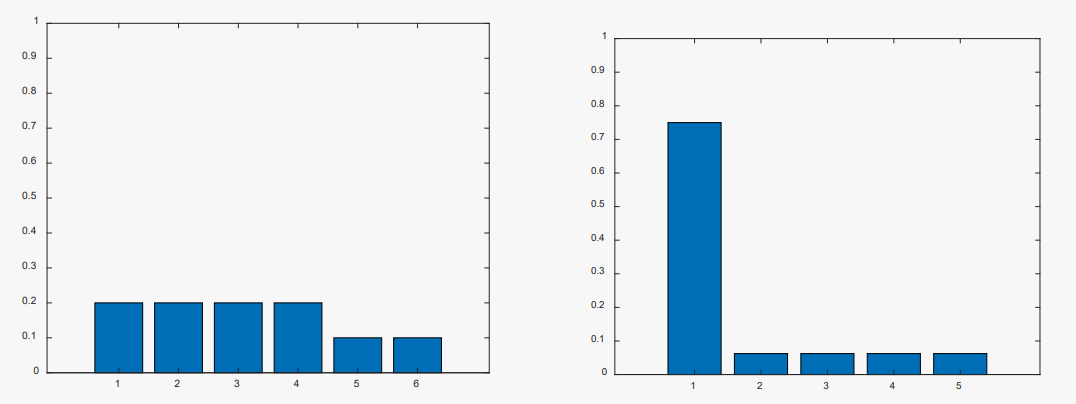
\includegraphics[scale=0.3]{prob1_histos.png}
    \end{figure}

    A. [4 points] Calculate the entropy for each variable.\\
    B. [4 points] Intuitively how can you tell which variable has a higher entropy without
    calculating the entropy numerically? What does higher entropy mean?

    \subsection{Answer}

    A. The entropy for each variable is given by:

    \begin{align*}
        H(p) &= -\sum_{i=1}^6 p_i \log_2 p_i \\
        &= -\left( 0.2 \log_2 0.2 + 0.2 \log_2 0.2 + 0.2 \log_2 0.2 + 0.2 \log_2 0.2 + 0.1 \log_2 0.1 + 0.1 \log_2 0.1 \right) \\
        &= -(4*0.2 \log_2 0.2 + 2*0.1 \log_2 0.1) \\
        &= 2.5219
    \end{align*}

    {\setlength{\mathindent}{1cm}
    \begin{align*}
        H(q) &= -\sum_{i=1}^5 q_i \log_2 q_i \\
        &= -\left( 0.75 \log_2 0.75 + 4*0.0625 \log_2 0.0625 \right) \\
        &= 1.3112
    \end{align*}}

    B. Entropy is defined as the lack of expected information, or the 
    `surprise'/uncertainty of a random variable. 
    We can tell that $q$ has a higher entropy than $p$ without calculating the entropy,
    because the histogram for $q$ shows that there is a `surprising' value of 0.75, which
    goes against the trend of the other values (which are all 0.0625). On the other hand,
    the histogram for $p$ shows that all the values are fairly close to each other. In general,
    higher entropy means that the random variable has more uncertainty,
    so the likelihood of encountering a value closer to the expected value is lower.



\end{homeworkProblem}

\nobreak\extramarks{Problem 2}{}\nobreak{}

\pagebreak

\begin{homeworkProblem}[Problem 2]
    \begin{figure}[h!]
        \centering
        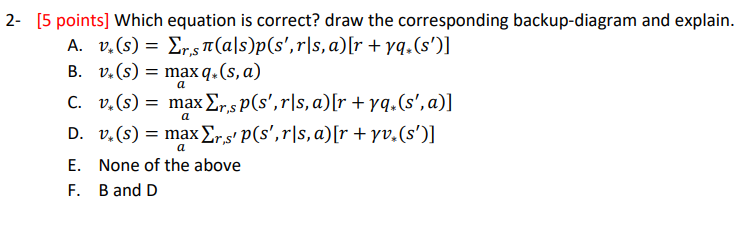
\includegraphics[scale=0.5]{prob2_prompt.png}
    \end{figure}

    \subsection{Answer}

    Option F (B and D) is correct.\\

    I have drawn the backup diagram for $v_*$ as given below:

    \begin{figure}[h!]
        \centering
        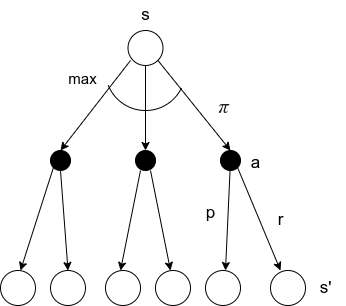
\includegraphics[scale=0.5]{vstar_drawio.png}
    \end{figure}

    \textbf{Explanation}

    $v_*$ is the optimal state-value function. The backup diagram for $v_*$ shows us that,
    if we start at a state s, we choose the action that maximizes the value of the state-action
    pair, and then we take the action. The action choice is taken using our current policy,
    $\pi$. Once we take the action, we end up in a new state, $s'$, and we get a reward, $r$.
    The resultant state $s'$ as well as the reward $r$ are chosen according
    to the dynamics of the environment, $p(s', r | s, a)$, which is not something we can control.
    In summary, the optimal state value function chooses the action that maximizes the value
    of the state-action value.\\

\end{homeworkProblem}

\nobreak\extramarks{Problem 2}{}\nobreak{}

\pagebreak

\nobreak\extramarks{Problem 3}{}\nobreak{}

\begin{homeworkProblem}[Problem 3]
    Consider a vehicle with 4 actions (left, right, up, down). There's no uncertainty in the outcome
    of the action (i.e. when left is commanded, the left state is achieved). The actions that cause
    the vehicle outside the grid, leave the state unchanged.
    The reward for all transition is -1 except when the goal is reached where the reward is zero.
    Discount factor $\gamma = 1$.\\
    The figure on left shows the name of the states and figure on the right shows the state-value
    $V(s)$, for each state under a uniform random policy.

    \begin{figure}[h!]
        \centering
        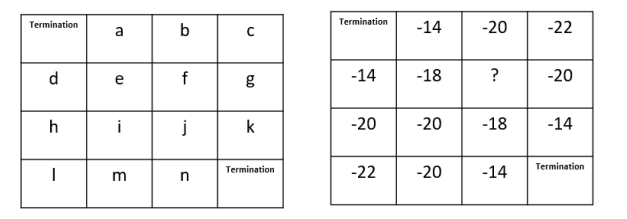
\includegraphics[scale=0.5]{prob3_prompt.png}
    \end{figure}

    A. [4 points] What is $q(k, down)$?\\
    B. [4 points] What is $q(g, down)$?\\
    C. [4 points] What is $V(f)$?\\

    \subsection{Answer}

    \textbf{A.} We know the equation for $q(s, a)$ is given by,

    \begin{align*}
        q(s, a) &= \sum_{s', r} p(s', r | s, a) \left[ r + \gamma V(s') \right]
    \end{align*}

    We can calculate $q(k, down)$ as follows:

    \begin{align*}
        q(k, down) &= \sum_{s', r} p(s', r | k, down) \left[ r + \gamma V(s') \right] \\
        &= 1 \left[ 0 + 1 \cdot 0 \right]\\
        &= 0
    \end{align*}

    \textbf{B.} We can calculate $q(g, down)$ as follows:

    \begin{align*}
        q(g, down) &= \sum_{s', r} p(s', r | g, down) \left[ r + \gamma V(s') \right] \\
        &= 1 \left[ -1 + 1 \cdot -14 \right]\\
        &= -15
    \end{align*}

    \textbf{C.} We know the equation for $V(s)$ is given by,

    \begin{align*}
        V(s) &= \sum_{a} \pi(a | s) q(s, a)
    \end{align*}
    
    We can calculate $V(f)$ as follows:

    \begin{align*}
        V(f) &= \sum_{s', r} p(s', r | f, \pi(f)) \left[ r + \gamma V(s') \right] \\
        &= 0.25 \left[ -1 + 1 \cdot -18 \right] + 0.25 \left[ -1 + 1 \cdot -20 \right] + 0.25 \left[ -1 + 1 \cdot -20 \right] + 0.25 \left[ -1 + 1 \cdot -18 \right]\\
        &= 0.25 \left[ -19 \right] + 0.25 \left[ -21 \right] + 0.25 \left[ -21 \right] + 0.25 \left[ -19 \right]\\
        &= 0.25 \left[ -80 \right]\\
        &= -20
    \end{align*}
    
\end{homeworkProblem}

\pagebreak

\nobreak\extramarks{Problem 4}{}\nobreak{}

\begin{homeworkProblem}[Problem 4]
    \begin{figure}[h!]
        \centering
        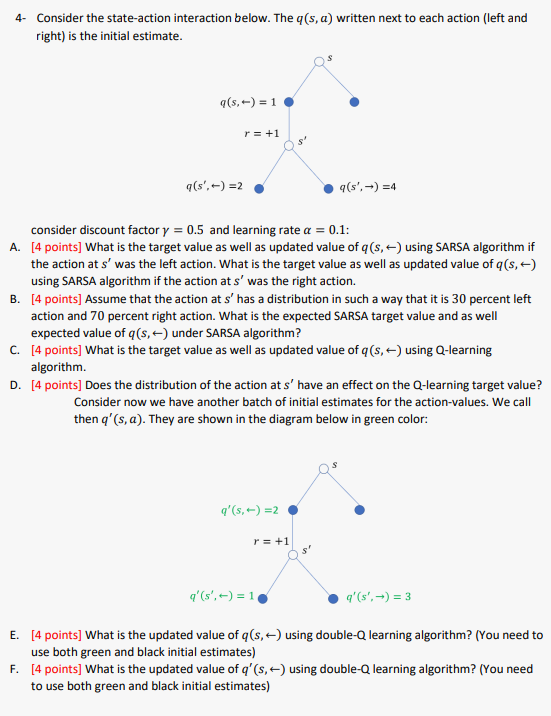
\includegraphics[scale=0.8]{prob4_prompt.png}
    \end{figure}

    \subsection{Answer}

    \textbf{A.} The target value for SARSA is given by
    $R + \gamma Q(S_{t+1}, A_{t+1})$.\\
    The update rule for SARSA is given by
    $Q(S_t, A_t) \leftarrow Q(S_t, A_t) + \alpha \left[ target - Q(S_t, A_t) \right]$.\\

    \textit{For left action at $s'$}:\\
    The target SARSA value at $q(s, left)$ is given by $1 + 0.5 \cdot 2 = 2$\\
    The update value for SARSA is given by $1 + 0.1 \cdot (2 - 1) = 1.1$\\

    \textit{For right action at $s'$}:\\
    The target SARSA value at $q(s, right)$ is given by $1 + 0.5 \cdot 4 = 3$\\
    The update value for SARSA is given by $1 + 0.1 \cdot (3 - 1) = 1.2$\\

    \vspace{0.75cm}

    \textbf{B.} The target value for Expected SARSA is given by
    $R + \gamma \sum_a \pi(a | S_{t+1}) Q(S_{t+1}, a)$.\\
    The update rule for Expected SARSA is given by
    $Q(S_t, A_t) \leftarrow Q(S_t, A_t) + \alpha \left[ target - Q(S_t, A_t) \right]$.\\

    The policy distribution for $s'$ is given by $\pi(left | s') = 0.3$ and $\pi(right | s') = 0.7$.\\
    
    The target Expected SARSA value at $q(s, left)$ is given by
    $1 + 0.5 (0.3 \cdot 2 + 0.7 \cdot 4) = 2.7$\\
    The update value for Expected SARSA is given by $1 + 0.1 \cdot (2.7 - 1) = 1.17$\\

    \vspace{0.5cm}

    \textbf{C.} The target value for Q-learning is given by
    $R + \gamma \max_a Q(S_{t+1}, a)$.\\
    The update rule for Q-learning is given by
    $Q(S_t, A_t) \leftarrow Q(S_t, A_t) + \alpha \left[ target - Q(S_t, A_t) \right]$.\\

    The target Q-learning value at $q(s, left)$ is given by $1 + 0.5 \cdot 4 = 3$\\
    The update value for Q-learning is given by $1 + 0.1 \cdot (3 - 1) = 1.2$\\

    \vspace{0.6cm}

    \textbf{D.} The distribution of the action at $s'$ does not affect the target value for Q-learning,
    because the target value for Q-learning is given by $R + \gamma \max_a Q(S_{t+1}, a)$, which
    does not depend on the action distribution at $s'$.\\

    \vspace{0.5cm}

    \textbf{E.} With the new batch of initial estimates, and applying double Q-learning,\\
    our $Q_1$ target is given by
    $R + \gamma Q_2(S_{t+1}, \arg\max_a Q_1(S_{t+1}, a))$\\
    and our $Q_2$ target is given by
    $R + \gamma Q_1(S_{t+1}, \arg\max_a Q_2(S_{t+1}, a))$\\

    The update rule for $Q_1$ is given by
    $Q_1(S_t, A_t) \leftarrow Q_1(S_t, A_t) + \alpha \left[ targetQ_1 - Q_1(S_t, A_t) \right]$.\\
    The update rule for $Q_2$ is given by
    $Q_2(S_t, A_t) \leftarrow Q_2(S_t, A_t) + \alpha \left[ targetQ_2 - Q_2(S_t, A_t) \right]$.\\

    The target value for $q(s, left)$ is given by $1 + 0.5 \cdot q'(s', right) = 1 + 0.5 \cdot 3 = 2.5$\\
    The update value for $q(s, left)$ is given by $1 + 0.1 \cdot (2.5 - 1) = 1.15$\\
    
    \textbf{F.}
    
    The target value for $q'(s, left)$ is given by $1 + 0.5 \cdot q(s', right) = 1 + 0.5 \cdot 4 = 3$\\
    The update value for $q'(s, left)$ is given by $2 + 0.1 \cdot (3 - 2) = 2.1$\

\end{homeworkProblem}

\pagebreak

\nobreak\extramarks{Problem 5}{}\nobreak{}

\begin{homeworkProblem}[Problem 5]
    As we discussed, n-step off-policy return via bootstrapping can be written as:
    \begin{align}
        G_{t:h} = \rho_t \left( R_{t+1} + \gamma G_{t+1:h} \right) 
    \end{align}
    where $\rho_t = \frac{\pi(A_t | S_t)}{b(A_t | S_t)}$
    is the importance sampling ratio between target and behavior policy.\\
    Using control variates, the return can be written as:
    \begin{align}
        G_{t:h} = \rho_t \left( R_{t+1} + \gamma G_{t+1:h} \right) + (1 - \rho_t) V_{h-1} (S_t)
    \end{align}
    • [8 points] Prove that introducing the control variates in equation (2) does not add any
    bias to the original return (i.e.\ equation (1)) in expectation.

    \subsection{Answer}

    If equation (2) does not add any bias to the original return, then we would be able to state that,
    \begin{align}\label{prob5toprove}
        \EX [ \rho_t \left( R_{t+1} + \gamma G_{t+1:h} \right) ] = \EX [ \rho_t \left( R_{t+1} + \gamma G_{t+1:h} \right) + (1 - \rho_t) V_{h-1} (S_t) ]
    \end{align}

    This is what we have to prove. Let us first consider the right hand side of the equation (\ref{prob5toprove}).
    We can expand it as follows:
    \begin{align*}
        &\EX [ \rho_t \left( R_{t+1} + \gamma G_{t+1:h} \right)] + \EX[(1 - \rho_t) V_{h-1} (S_t) ]\\
        = &\EX [ \rho_t \left( R_{t+1} + \gamma G_{t+1:h} \right)] + \EX[(V_{h-1} (S_t) - \rho_t V_{h-1} (S_t) ]\\
        = &\EX [ \rho_t \left( R_{t+1} + \gamma G_{t+1:h} \right)] + \EX[V_{h-1} (S_t)] - \EX[\rho_t V_{h-1} (S_t) ]
    \end{align*}

    However, $\rho_t$ is independent of $V_{h-1} (S_t)$ because the ratio of the target policy
    and the behavior policy is independent of the value function. Therefore, we can further
    write the right hand side of the equation (\ref{prob5toprove}) as,
    \begin{align}\label{prob5rhs}
        \EX [ \rho_t \left( R_{t+1} + \gamma G_{t+1:h} \right)] + \EX[V_{h-1} (S_t)] - \EX[\rho_t] \EX[V_{h-1} (S_t) ]
    \end{align}

    Furthermore, the expectation of the importance sampling ratio is given by,

    \begin{align*}
        \EX[\rho_t] &= \EX \left[ \frac{\pi(A_t | S_t)}{b(A_t | S_t)} \right]
        = \sum_{a} b(a | S_t) \frac{\pi(a | S_t)}{b(a | S_t)} = \sum_{a} \pi(a | S_t) = 1
    \end{align*}

    Which we can substitute into equation (\ref{prob5rhs}) to get,

    \begin{align*}
        &\EX [ \rho_t \left( R_{t+1} + \gamma G_{t+1:h} \right)] + \EX[V_{h-1} (S_t)] - \EX[V_{h-1} (S_t) ]\\
        = &\EX [ \rho_t \left( R_{t+1} + \gamma G_{t+1:h} \right)]
    \end{align*}

    Which is the same as the left hand side of the equation (\ref{prob5toprove}). Therefore,
    we have proved that equation (2) does not add any bias to the original return in expectation.

\end{homeworkProblem}

\pagebreak

\nobreak\extramarks{Problem 6}{}\nobreak{}

\begin{homeworkProblem}[Problem 6]
    [8 points] If you were to design an algorithm called TD-search by modifying the Monte-Carlo
    Tree Search, how do you go about it. In particular, which part of the MCTS you would modify
    and how?

    \subsection{Answer}

    TD methods use bootstrapping, whereas MCTS does not. Therefore, to design TD-search by
    modifying MCTS, we can incorporate bootstrapping into MCTS.\\

    Specifically, we can modify the simulation phase of MCTS to use TD methods.

\end{homeworkProblem}

\pagebreak

\nobreak\extramarks{Problem 7}{}\nobreak{}

\begin{homeworkProblem}[Problem 7]
    \begin{figure}[h!]
        \centering
        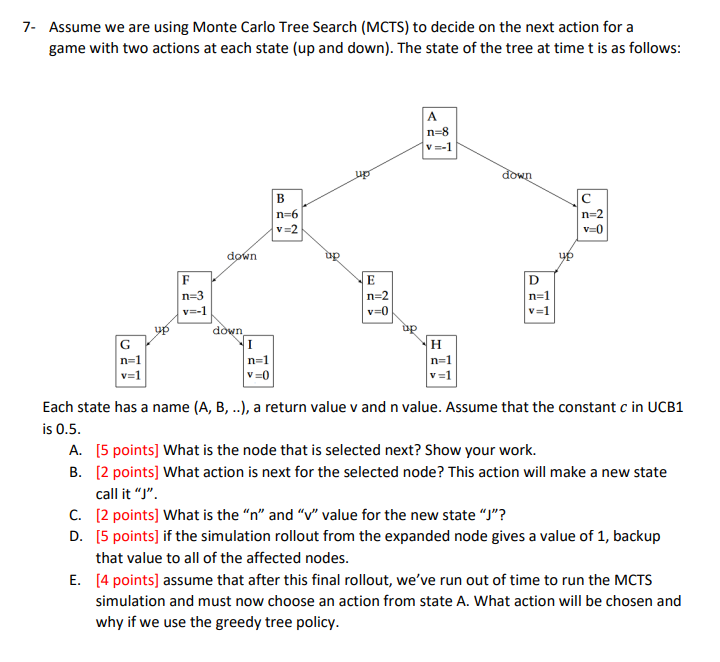
\includegraphics[scale=0.5]{prob7_prompt.png}
    \end{figure}

    \subsection{Answer}

    \textbf{A.} We can use the following flowchart to choose the next node:

    \begin{figure}[h!]
        \centering
        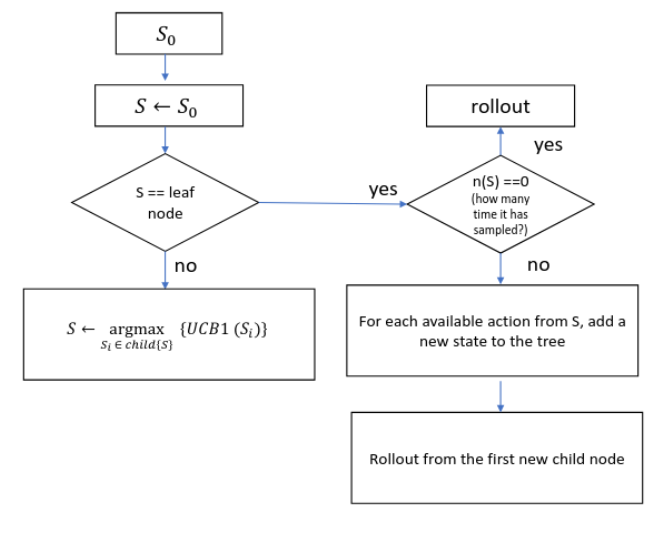
\includegraphics[scale=0.37]{prob7_flowchart.png}
    \end{figure}

    The UCB1 formula is given by,

    \begin{align*}
        UCB1(S_i) = \frac{v_i}{n_i} + C \sqrt{\frac{\ln N_i}{n_i}}
    \end{align*}

    Where,\\
    $n_i$ is the number of times we have visited node $S_i$,\\
    $N_i$ is the number of times we have visited the parent of node $S_i$,\\
    $v_i$ is the value of node $S_i$, and\\
    $C$ is a constant that we choose.\\

    Starting at A, we choose B because by the UCB1 algorithm,

    \begin{align*}
        \frac{2}{6} + 0.5 \sqrt{\frac{\ln 8}{6}} &> \frac{0}{2} + 0.5 \sqrt{\frac{\ln 8}{2}}\\
        0.62 &> 0.51
    \end{align*}

    Then, at B, we pick E because,

    \begin{align*}
        \frac{-1}{3} + 0.5 \sqrt{\frac{\ln 6}{3}} &< \frac{0}{2} + 0.5 \sqrt{\frac{\ln 6}{2}}\\
        0.053 &< 0.473
    \end{align*}

    Then, at E, we pick H because that is the only option. It is possible that H is
    the only option because there is no valid down action from E.\\

    Hence, H is the next node we pick.

    \vspace{0.5cm}

    \textbf{B.} At H, we assume that both up and down actions are valid, since
    the prompt of this question does not specify otherwise. Therefore, we add
    both up and down nodes from H. Since the first action is up, we choose it.
    This up action creates a new state, which is the `J' node.\\

    \textbf{C.} The `n' and `v' of J are 0 and 0 currently because we have not
    visited J yet, and we have not rolled out from it yet.\\

    \textbf{D.} The simulation from J gives a value of 1. So now we can
    backup the tree and update the `n' and `v' of J and its ancestors. The
    new values are given below:

    J\@: $n = 1$, $v = 1$\\
    H\@: $n = 2$, $v = 2$\\
    E\@: $n = 3$, $v = 1$\\
    B\@: $n = 7$, $v = 3$\\
    A\@: $n = 9$, $v = 0$\\

    \textbf{E.} Now that we have run out of time, we compare the up and down
    actions at A. With up, we reach B, which has an average reward is $3/7 = 0.42$.
    With down, we reach C, which has an average reward of $0/2 = 0$. Therefore we
    choose up because in the greedy tree policy we choose the action that maximizes
    the average reward.\\

\end{homeworkProblem}

\end{document}